\subsubsection{Fronts bidirectionnels et reconstruction du chemin}\label{sec:biwfa}
Hirschberg choisit la coupe sur une ligne fixée à l’avance. Dans BiWFA, de Marco-Sola et ses coauteurs, la rencontre de deux fronts détermine la coupe~\cite{biwfa}. Pour les coûts unitaires de l’expérience, les fronts partent des extrémités opposées de l’alignement et cherchent un chevauchement sur une même diagonale. Une jonction optimale \((i,j)\) scinde les chaînes \(A,B\) en deux sous-problèmes dont les coûts se composent,
\[
 d(A,B)=d\bigl(A[0:i],B[0:j]\bigr)+d\bigl(A[i:m],B[j:n]\bigr).
\]
Le mode score s'arrête lorsque la jonction ou l'extrémité est atteinte. Pour restituer le chemin, BiWFA résout les sous-problèmes et assemble leurs opérations. Avec \(s=d(A,B)\ge1\) et \(L=\max(m,n)\), la borne de temps est \(O(Ls)\) et celle de mémoire de travail des fronts \(O(s)\). Le RSS comprend aussi les entrées, les copies et le chemin rendu. La version mesurée utilise un front unidirectionnel auxiliaire sur les petits sous-problèmes.

L'algorithme~\ref{alg:biwfa} décrit cette décomposition pour le coût unitaire. La figure~\ref{fig:jonction} donne un chemin de coût deux. La substitution précède la jonction et l'insertion la suit.
\begin{algorithm}[htbp]
\caption{Reconstruction d'un chemin par fronts bidirectionnels}\label{alg:biwfa}
\begin{algorithmic}[1]
\Require Strings \(A,B\), unit edit costs
\Ensure Optimal operation sequence \(P\)
\If{\Call{BaseCase}{$A,B$}}
  \State \Return \Call{UnidirectionalTrace}{$A,B$}
\EndIf
\State \((i,j)\gets\Call{OptimalOverlap}{A,B}\) \Comment{forward and reverse wavefronts}
\State \(P_L\gets\Call{BiWFA}{A[0:i],B[0:j]}\)
\State \(P_R\gets\Call{BiWFA}{A[i:m],B[j:n]}\)
\State \Return \(P_L\mathbin{\Vert}P_R\)
\end{algorithmic}
\end{algorithm}
\schema{jonction}{Une jonction optimale sépare la substitution du préfixe et l'insertion du suffixe sur deux chaînes courtes.}{fig:jonction}{src/libraries/wfa2/wfa_adapter.c}

\begin{figure}[htbp]\centering
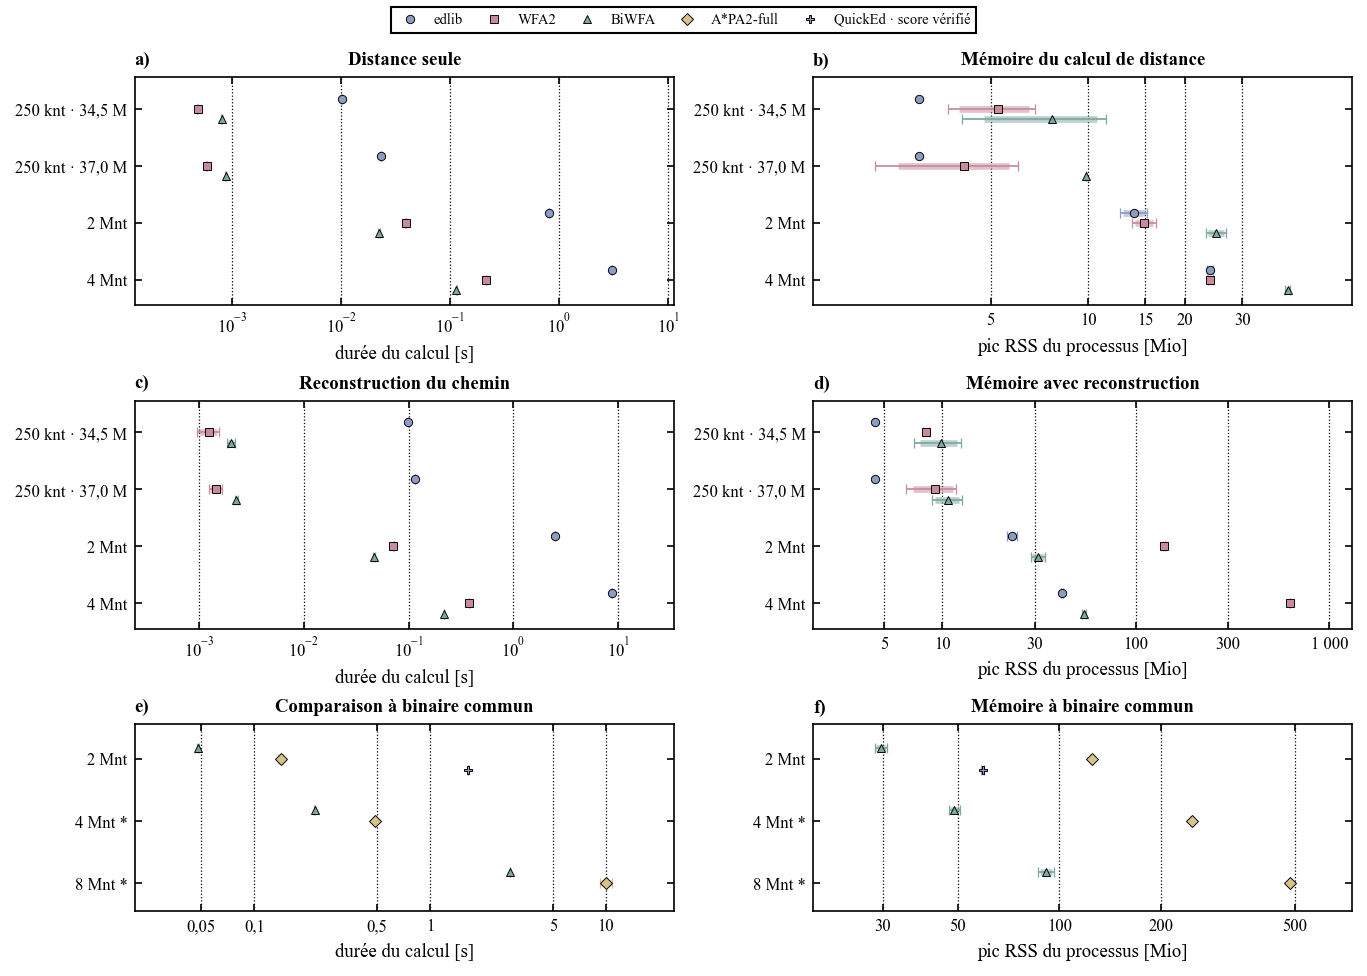
\includegraphics[width=.97\linewidth,height=.44\textheight,keepaspectratio]{../figures/comparison/biwfa_humain.png}
\sourcefig{bench/human/algorithms/study.py}
\caption{Les rapports de temps et de mémoire entre WFA2 et BiWFA distinguent le score et la reconstruction sur un cœur EPYC. Un rapport supérieur à un favorise BiWFA. Le tableau donne les temps d’une seconde allocation. Le terme « échéance » indique un arrêt du processus à 120\,s, chauffe comprise.}\label{fig:biwfa}
\end{figure}
La figure~\ref{fig:biwfa} compare des appels complets après échauffement, sur cinq processus indépendants par cas. Les fenêtres se recouvrent en partie. À quatre millions de bases et \(s=12\,482\), BiWFA rend le chemin en \(218{,}72\pm1{,}00\)\,ms avec un pic RSS moyen de 54,02\,Mio. WFA2 unidirectionnel prend \(375{,}90\pm2{,}35\)\,ms et 627,02\,Mio pour le même résultat. La moyenne des rapports appariés de temps vaut 1,719 (IC à 95\,\% de 1,707 à 1,730). Sur les deux loci de 250\,000 bases, WFA2 unidirectionnel termine en \(1{,}25\pm0{,}24\) et \(1{,}45\pm0{,}16\)\,ms. BiWFA prend \(2{,}03\pm0{,}13\) et \(2{,}28\pm0{,}06\)\,ms.

\begin{samepage}
Pour le score seul, le classement en mémoire s’inverse (panneaux a et b). À quatre millions de bases, le score seul occupe 23,87\,Mio avec WFA2, qui réutilise ses fronts en mémoire circulaire, et 41,46\,Mio avec BiWFA. Un relevé séparé sur la fenêtre de deux millions de bases compte 62 choix de sous-intervalle pendant la reconstruction BiWFA et aucun en mode score seul.\par
\end{samepage}

Un second banc utilise le même cœur pour les méthodes comparées à taille fixée. A*PA2 et BiWFA rendent le chemin. L'adaptateur QuickEd vérifie son chemin en interne et rend le score. À huit millions de bases, A*PA2 de Groot Koerkamp~\cite{astar} prend \(10{,}040\pm0{,}628\)\,s et BiWFA \(2{,}845\pm0{,}008\)\,s. À deux millions, QuickEd de Doblas et ses coauteurs~\cite{quicked}, avec contrôle du chemin, prend \(1{,}6391\pm0{,}0002\)\,s. Les processus QuickEd sur quatre et huit millions de bases atteignent la limite de 120\,s, lecture et échauffement compris.

\synthese{Sur la fenêtre de quatre millions de bases, le pic RSS de WFA2 pour restituer le chemin vaut 11,61 fois celui de BiWFA en moyenne sur les cinq rapports appariés. Les deux méthodes donnent le même coût.}

\subsubsection{Alignement du bras long du chromosome humain}\label{sec:bras}
Quatre fenêtres emboîtées du bras long du chromosome 21 partagent la même borne gauche, la base 14\,000\,100 de GRCh38 en coordonnées commençant à zéro. Leurs longueurs de référence valent 8, 16, 24 et 32 millions de bases. Leurs distances globales valent respectivement 47\,493, 89\,448, 133\,991 et 266\,220 éditions. Les chemins optimaux peuvent changer quand la borne droite se déplace. La soustraction de deux scores emboîtés ne suffit donc pas à localiser les éditions.

La fenêtre de 32 millions de bases contient 50\,160 caractères \texttt{N} dans GRCh38. CHM13 contient 31\,347 bases de plus et aucun \texttt{N}. Transformer la première chaîne en la seconde impose au moins une substitution ou une délétion pour chacun des \texttt{N}, ainsi qu'au moins 31\,347 insertions. Ces opérations distinctes donnent la borne \(d\ge50\,160+31\,347=81\,507\) pour les chaînes déposées.

\chart{comparison/bras_chromosome_biwfa.png}{BiWFA et WFA2 calculent le score sur quatre fenêtres emboîtées du bras long du chromosome 21. BiWFA restitue aussi un chemin sur chaque fenêtre. Les deux mesures d'Edlib (score seul et chemin) portent sur la fenêtre de 8~Mnt.}{fig:bras}{bench/human/algorithms/arm.py}
Les quatre tailles de la figure~\ref{fig:bras} occupent chacune un cœur distinct de l’EPYC. Les méthodes se succèdent sur ce cœur dans un ordre tiré par bloc. Chaque cas comporte cinq processus après échauffement. À 32 millions de bases, BiWFA calcule le score en \(45{,}62\pm0{,}22\)\,s et restitue le chemin en \(89{,}77\pm0{,}11\)\,s. Le pic RSS moyen atteint respectivement 272,83 et 311,17\,Mio. WFA2 unidirectionnel donne le score en \(102{,}04\pm0{,}91\)\,s avec 143,81\,Mio. Les fronts bidirectionnels se rejoignent avant que l'un d'eux atteigne le score total. Le gain en temps coïncide ici avec une hausse du pic résident.

\synthese{La restitution du chemin par BiWFA prend \(2{,}876\pm0{,}023\)\,s sur 8 millions de bases. Entre 8 et 32 millions de bases, la distance augmente d’un facteur 5,61 et le temps moyen d’un facteur 31,2. Ces fenêtres emboîtées font varier à la fois la longueur et la distance.}
